\section{ОБЗОР ЛИТЕРАТУРЫ}
\label{sec:domain}

%=======================================================================================================================
%В обзоре литературы обычно содержится краткий анализ литературных источников различных типов,
%использованных в процессе работы над дипломным проектом.
%Здесь приводятся основные сведения, почерпнутые из литературы.
%Возможен анализ патентной чистоты.
%=======================================================================================================================
В обзоре литературы содержится информация о технологиях, которые будут использованы в процессе написания дипломного проектирования.
%Помимо самих технологий и конкретных примеров, реализу


\subsection{Python}\label{subsec:domain:python}
В современном мире скорость разработки программного обеспечения играет важную роль, экономя не только время, но и средства, затраченные на разработку.
Таким свойством обладает один из высокоуровневых языков программирования -- Python.
Помимо высокой скорости разработки Python также обладает следующими свойствами:
\begin{itemize}
    \item Большая стандартная библиотека.
    Python поставляется с обширной стандартной библиотекой, включающей в себя множество модулей и инструментов для различных задач, таких как работа с файлами, сетевое программирование, обработка данных и многое другое.
    \item Богатая экосистема библиотек и фреймворков.
    Python обладает обширной экосистемой сторонних библиотек и фреймворков, предназначенных для различных целей, включая веб-разработку, научные вычисления, машинное обучение, обработку изображений и многое другое.
    \item Динамическая типизация.
    Python является языком с динамической типизацией, что упрощает процесс разработки.
    \item Автоматическое управление памятью.
    Python автоматически управляет памятью, что облегчает работу с динамическими структурами данных и снижает вероятность утечек памяти.
\end{itemize}

Основными направлениями разработки на Python являются веб-приложения, Big Data, машинное обучение.

%=======================================================================================================================

\subsection{Веб-приложение}\label{subsec:domain:web-application}
Веб-приложением принято называть программное обеспечение, предназначенное для выполнения определенных функций или задач через веб-браузер.
Веб-приложения отличаются от традиционных десктопных приложений тем, что не требуют установки на компьютер пользователя и могут быть запущены в любом совместимом веб-браузере.
Основными характеристиками веб-приложения являются:
\begin{itemize}
    \item Клиент-серверная архитектура.
    Веб-приложение включает в себя клиентскую часть и серверную части.
    К клиентской части относится то, что видит пользователь, например веб-страница.
    Серверная часть хранит данные и выполняется операции, обрабатывая запросы, поступаемые с клиентской части.
    Взаимодействие между клиентом и сервером происходит посредством HTTP или HTTPS -- протоколов прикладного уровня, относительно модели OSI.
    \item Доступность через интернет.
    Веб-приложения доступны для пользователей через интернет, что позволяет им использовать приложение из любой точки мира, где есть доступ к сети.
    \item Обновление и сопровождение.
    Одним из преимуществ веб-приложений является возможность централизованного обновления и сопровождения.
    Изменения в приложении могут быть внесены на сервере и автоматически доступны всем пользователям без необходимости обновления на стороне клиента.
\end{itemize}
    \nomenclaturex{HTTP}{HyperText Transfer Protocol}{протокол передачи гипертекста}
    \nomenclaturex{HTTPS}{HyperText Transfer Protocol Secure}{безопасный протокол передачи гипертекста}
    \nomenclaturex{OSI}{Open Systems Interconnection}{взаимосвязь открытых систем}

%=======================================================================================================================

\subsection{Веб-фреймворк}\label{subsec:domain:web-framework}
Говоря простыми словами, фреймворк -- это набор инструментов, ускоряющих разработку приложений.
Веб-фреймворк упрощает разработку и избавляет от необходимости написания рутинного кода при создании динамических веб-сайтов, сетевых приложений, сервисов или ресурсов.

Для языка программирования Python существует несколько популярных веб-фреймворков:
\begin{itemize}
    \item Django
    \item Django Rest Framework
    \item Flask
    \item FastAPI
\end{itemize}

На рисунке 1.1 изображено количество запросов, которое способен обработать каждый из фреймворков за секунду.
%~\ref{fig:domain:frameworks-rps} !!!

\begin{figure}[ht]
    \centering
    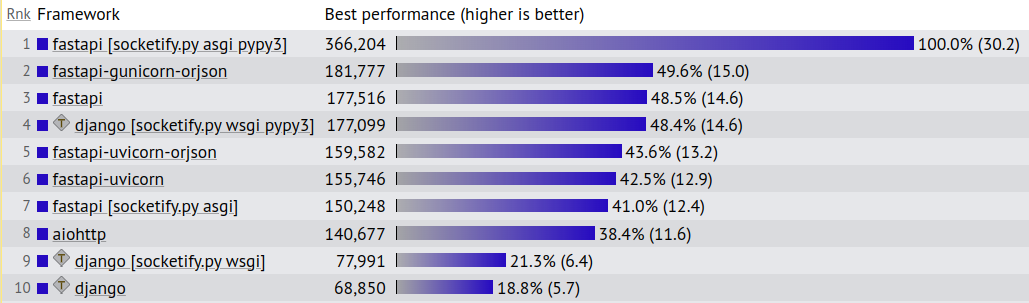
\includegraphics[width=.8\linewidth]{images/frameworks_rps}
    \caption{Сравнение RPS веб-фреймворков}
    \label{fig:domain:frameworks-rps}
\end{figure}

RPS -- это метрика, измеряющая количество HTTP запросов, которые веб-приложение или веб-сервер способен обработать за секунду.
Фреймворки веб-разработки могут различаться по производительности в обработке запросов в секунду в зависимости от различных факторов, таких как архитектура, используемые технологии или оптимизации.


    \nomenclaturex{RPS}{Requests Per Second}{запросы в секунду}

%=======================================================================================================================

\subsubsection{Django и Django Rest Framework}\label{subsubsec:domain:django--django-rest-framework}
Одним из популярных веб-фреймворком на Python является Django.
Django основан на модели MVC и знаменит большим количеством функционала «из коробки».
Среди готового функционала выделяют Django ORM и Django Admin Panel.

Помимо этого Django имеет встроенную защиту от таких уязвимостей как CSRF-атаки, SQL-инъекции, XSS-атаки и других видов угроз.
Django также имеет расширение под названием Django Rest Framework, которое направлено ускорить разработку REST API.

    \nomenclaturex{REST}{REpresentational State Transfer}{передача репрезентативного состояния}
    \nomenclaturex{API}{(Application Programming Interface}{интерфейс программирования приложения}
    \nomenclaturex{MVC}{Model View Controller}{модель, отображение, контроллер}
    \nomenclaturex{ORM}{Object Related Mapper}{объектно-реляционное отображение}
    \nomenclaturex{CSRF}{Cross-Site Request Forgery}{межсайтовая подделка запроса}
    \nomenclaturex{SQL}{Structured Query Language}{язык структурированных запросов}
    \nomenclaturex{XSS}{Cross-Site Scripting}{межсайтовый скриптинг}

%\subsubsection{Django ORM}\label{subsec:domain:django-orm}
Django ORM -- это инструмент, предоставляемый фреймворком Django для работы с базой данных.
Он позволяет разработчикам взаимодействовать с базой данных, используя объектно-ориентированный подход,
что делает процесс работы с данными более удобным и интуитивным.

Основными концепциями Django ORM являются:
\begin{itemize}
    \item Модели данных.
    Django ORM позволяет описывать структуру данных с помощью моделей Django.
    Модель представляет собой класс Python, который соответствует таблице в базе данных.
    Каждое поле модели соответствует столбцу в таблице.
    \item ORM запросы.
    Django ORM предоставляет мощный интерфейс для выполнения запросов к базе данных, используя высокоуровневый язык запросов, похожий на SQL,
    но более удобный для использования в Python коде.
    С помощью ORM запросов можно выполнять операции выборки, вставки, обновления и удаления данных.
    \item Ленивая загрузка данных.
    Django ORM использует концепцию ленивой загрузки данных, что означает,
    что данные из базы данных извлекаются только в тот момент, когда они реально нужны при выполнении кода.
    Это позволяет оптимизировать производительность приложения и избегать излишнего запроса данных.
    \item Отношения между моделями.
    Django ORM поддерживает различные типы отношений между моделями,
    такие как один-к-одному, один-ко-многим и многие-ко-многим.
    Это позволяет создавать сложные структуры данных и эффективно организовывать взаимосвязанные данные.
    Миграции базы данных.
    Django ORM автоматически создает и применяет миграции базы данных на основе изменений в моделях Django.
    Это позволяет легко обновлять схему базы данных без необходимости вручную изменять структуру таблиц.
    \item Интеграция с административной панелью.
    Django ORM интегрирован с административной панелью Django, позволяя разработчикам управлять данными, хранящимися в базе данных, через веб-интерфейс без необходимости написания дополнительного кода.
\end{itemize}


\subsubsection{FastAPI}\label{subsubsec:domain:fastapi}
FastAPI -- это современный фреймворк для создания веб-приложений и API на языке Python.
Он известен своей высокой производительностью, интуитивно понятным API, автоматической документацией и поддержкой типов данных, что делает его привлекательным выбором для быстрой и эффективной разработки веб-приложений и микросервисов.
Основными плюсами использования FastAPI являются:
\begin{itemize}
    \item Основан на стандартном Python.
    FastAPI построен поверх стандартного Python, используя синтаксис и инструменты, такие как аннотации типов и асинхронное программирование.
    Это делает его легким для понимания и использования для разработчиков, знакомых с Python.
    \item Автоматическая документация.
    FastAPI автоматически создает интерактивную документацию для вашего API на основе аннотаций типов и комментариев в коде.
    Это позволяет разработчикам легко понять структуру и использование API без дополнительной документации.
    \item Поддержка асинхронного программирования.
    FastAPI полностью совместим с асинхронным программированием, что позволяет создавать высокопроизводительные веб-приложения, способные обрабатывать тысячи запросов одновременно без блокировки потоков.
\end{itemize}

\subsubsection{Промежуточное ПО}\label{subsubsec:domain:middleware}
Промежуточное ПО (далее middleware) - это слой программного обеспечения, который располагается между клиентом и сервером (или между различными компонентами приложения) и обрабатывает запросы и ответы до того, как они достигнут конечного назначения.
В контексте Python веб-фреймворков оно реализуется на уровне между веб-сервером и веб-приложением.

Middleware обрабатывает запросы до того, как они достигнут приложения, и ответы до того, как они достигнут клиента.
Это позволяет выполнять дополнительные операции с данными, например, их изменение, анализ или фильтрацию.

Middleware используется для выполнения таких задач как:
\begin{itemize}
    \item Аутентификация и авторизация.
    Middleware может проверять аутентификацию пользователя и его доступ к определенным ресурсам, блокируя или разрешая доступ к ним.
    \item Логирование.
    Middleware может регистрировать информацию о запросах и ответах для анализа и мониторинга работы приложения.
    \item Обработка ошибок.
    Middleware может перехватывать и обрабатывать ошибки, возникающие при выполнении запросов, и возвращать соответствующие ответы.
\end{itemize}

Во многих фреймворках middleware организованы в цепочку, где каждый middleware может обрабатывать запрос и передавать его следующему middleware в цепочке.
В контексте языка программирования Python, такими фреймворками являются Django, Flask и другие.

%=======================================================================================================================

\subsection{REST}\label{subsec:domain:rest}
REST -- это архитектурный стиль, используемый для проектирования распределенных систем, таких как веб-сервисы.
REST опирается на принципы и ограничения, которые позволяют создавать гибкие, масштабируемые и удобные для использования веб-сервисы.

В контексте REST существует шесть принципов:
\begin{itemize}
    \item Ресурсы.
    В основе REST лежит концепция ресурсов - абстракций информации, представленной в системе.
    Ресурсы могут быть любыми объектами или сущностями, которые могут быть идентифицированы уникальным URI.
    \item HTTP методы.
    REST использует стандартные HTTP методы GET, POST, PUT и DELETE для выполнения операций над ресурсами.
    Каждый метод имеет свое назначение.
    GET используется для получения данных,
    POST - для создания новых ресурсов,
    PUT - для обновления существующих ресурсов,
    DELETE - для удаления ресурсов.
    \item Представление ресурсов.
    Ресурсы могут иметь различные представления, представленные в форматах JSON или XML.
    Клиенты могут запрашивать представления ресурсов, которые соответствуют их потребностям, используя HTTP заголовки Accept.
    \item Без состояния.
    Клиент и сервер взаимодействуют между собой без сохранения состояния на сервере.
    Каждый запрос от клиента к серверу должен содержать всю необходимую информацию для выполнения операции, что упрощает масштабирование системы и обеспечивает надежность.
    \item Ограниченный интерфейс.
    REST ограничивает интерфейс только на несколько универсальных методов HTTP, что позволяет упростить проектирование и поддержку веб-сервисов.
    \item Самоописываемые сервисы.
    REST сервисы должны быть самоописываемыми, что означает, что клиенты могут получить информацию о доступных ресурсах и операциях над ними, используя стандартные средства, например, заголовок OPTIONS.
\end{itemize}

Приложения, которые следуют всем шести принципам REST принято называть RESTfull.

    \nomenclaturex{URI}{Uniform Resource Identifier}{унифицированный идентификатор ресурса}
    \nomenclaturex{JSON}{JavaScript Object Notation}{обозначение объектов JavaScript}
    \nomenclaturex{XML}{eXtensible Markup Language}{расширяемый язык разметки}

%=======================================================================================================================

\subsection{JWT}\label{subsec:domain:jwt}
JWT -- это открытый стандарт RFC 7519, который определяет компактный и самодостаточный способ представления информации между двумя сторонами в формате JSON.
JWT состоит из трех частей, разделенных точками:
\begin{itemize}
    \item Header (заголовок).
    Содержит тип токена и алгоритм шифрования.
    \item Payload (полезная нагрузка).
    Содержит утверждения (claims), которые представляют собой утверждения о пользователе или о других данными.
    Примерами утверждений являются идентификатор пользователя (sub), срок действия (exp) и другие.
    \item Signature (подпись).
    Подпись, которая используется для проверки подлинности содержимого токена и его происхождения.
    Подпись вычисляется на основе заголовка, полезной нагрузки и секретного ключа, известного только серверу.
\end{itemize}

В общем виде структура JWT приведена на рисунке 1.2.

\begin{figure}[ht]
    \centering
    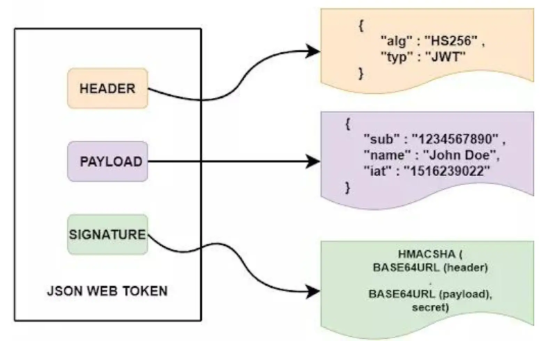
\includegraphics[width=.8\linewidth]{images/jwt_struct}
    \caption{Cтруктура JWT}
    \label{fig:domain:jwt-structure}
\end{figure}


    \nomenclaturex{JWT}{JSON Web Token}{JSON веб-токен}

%=======================================================================================================================

\subsection{PostgreSQL}\label{subsec:domain:postgresql}
PostgreSQL -- это мощная и открытая объектно-реляционная система управления базами данных, известная своей надежностью, расширяемостью и богатым набором функций.
Опыт использования данной базы данных был получен при проходении курса баз данных.
Ключевыми особенностями PostgreSQL являются:
\begin{itemize}
    \item Открытая и бесплатная.
    PostgreSQL распространяется под свободной лицензией, что позволяет использовать его бесплатно как в коммерческих, так и в некоммерческих проектах.
    Благодаря этому он широко распространен и популярен среди разработчиков по всему миру.
    \item Расширяемость.
    PostgreSQL предоставляет множество расширений и дополнений, позволяющих расширить его функциональность для удовлетворения различных потребностей.
    Это включает в себя расширения для полнотекстового поиска, географических операций, аналитики и других.
    \item Стандарты и соответствие.
    PostgreSQL строго следует стандартам SQL и поддерживает множество расширений ANSI SQL, что обеспечивает высокую совместимость с другими базами данных и упрощает перенос приложений между различными платформами.
    \item Масштабируемость и производительность.
    PostgreSQL поддерживает различные методы масштабирования, включая репликацию, разделение данных и партиционирование, что позволяет обеспечивать высокую производительность и доступность для приложений любого размера.
    \item Безопасность.
    PostgreSQL предоставляет множество функций для обеспечения безопасности данных, включая аутентификацию, авторизацию, шифрование и аудит.
    Это позволяет разработчикам создавать безопасные и надежные приложения, защищенные от различных угроз.
    \item Обширная документация и сообщество.
    PostgreSQL имеет обширную документацию, которая покрывает все аспекты его использования и настройки.
    Кроме того, существует активное сообщество пользователей и разработчиков, готовых помочь в решении любых вопросов и проблем.
\end{itemize}

PostgreSQL является мощной и гибкой СУБД, которая подходит для широкого спектра задач и проектов.
Благодаря своей открытости, надежности и богатому функционалу, он остается одним из наиболее популярных выборов для разработки и поддержки баз данных.
%!!!рисунок

%=======================================================================================================================

\subsection{MongoDB}\label{subsec:domain:mongodb}
MongoDB -- это распределенная, гибкая и масштабируемая система управления базами данных,
ориентированная на документы, которая позволяет хранить и обрабатывать данные в формате BSON.
В отличие от реляционных СУБД, документоориентированные СУБД хранят данные не в таблицах, а в коллекциях и не имеют срогой схемы данных.
MongoDB также обеспечивает горизонтальную масштабируемость, безопасность и аунтефикацию и
высокую производительность за счет использования индексов, кэширования и оптимизаций запросов.
Также имеется поддержка асинхронных запросов, что хорошо подходит для использования из FastAPI.

    \nomenclaturex{BSON}{Binary JavaScript Object Notation}{бинарное обозначение объектов JavaScript}
    \nomenclatureRus{СУБД}{Система Управления Базами Данных}

%=======================================================================================================================

\subsection{Микросервисная архитектура}\label{subsec:domain:microservices-arch}
Микросервисная архитектура -- это подход к проектированию и разработке программного обеспечения, в котором приложение разбивается на небольшие, независимые и взаимодействующие между собой сервисы.
Вместо создания монолитного приложения, где вся функциональность сосредоточена в одном приложении, микросервисная архитектура разделяет приложение на отдельные компоненты, каждый из которых представляет собой отдельный сервис.
Среди плюсов использования микросервисной архитектуры выделяют:
\begin{itemize}
    \item гибкость и масштабируемость;
    \item улучшенная отказоустойчивость;
    \item более быстрая разработка и поставка;
    \item простота масштабирования и сопровождения;
    \item лучшая изоляция и безопасность.
\end{itemize}

%=======================================================================================================================

\subsection{Брокеры сообщений}\label{subsec:domain:message-brokers}
Брокеры сообщений -- это программные компоненты, которые играют ключевую роль в асинхронной связи между различными приложениями или компонентами в распределенной системе.
Они обеспечивают надежную и эффективную доставку сообщений от отправителя к одному или нескольким получателям.
Говоря про ассинхронную связь подразумевается, что передаваемая информация хранится в так называемом буфере.
Этим буфером выступает очередь сообщений.
Сообщения помещаются в очередь производителем и забираются из неё потребителем, но сами производители и потребители не знаю друг о друге.
Модель взаимодействия производителей и потребителей приведена на рисунке 1.3.
%~\ref{fig:domain:mb-interaction-model}.

\begin{figure}[ht]
    \centering
    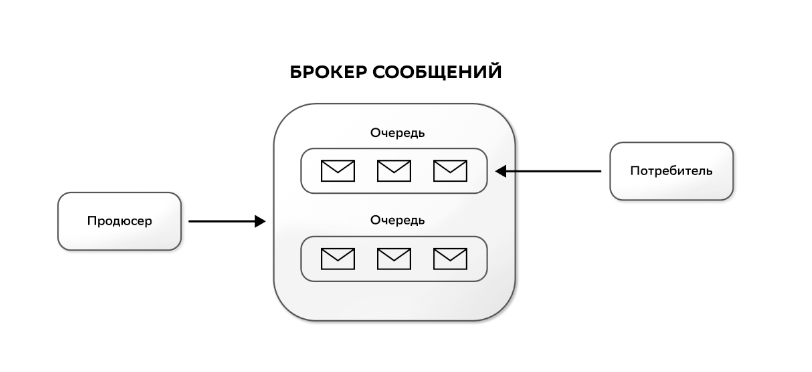
\includegraphics[width=.6\linewidth]{images/mb_interaction_model}
    \caption{Модель взаимодействия внутри брокера сообщений}
    \label{fig:domain:mb-interaction-model}
\end{figure}

%В таблице~\ref{table::domain::http-vs-mb} представлены основные различия между взаимодействием по HTTP и взаимодействием посредством брокеров сообщений.
%    \begin{longtable}{
%        | >{\raggedright}m{0.3\textwidth}
%        | >{\raggedright}m{0.35\textwidth}
%        | >{\raggedright\arraybackslash}m{0.35\textwidth}|}
%
%        \caption{Сравнение характеристик способов взаимодействия}
%        \label{table::domain::http-vs-mb} \\
%        \hline
%        \centering Характеристика
%        & \centering\arraybackslash Брокеры сообщений
%        & \centering\arraybackslash HTTP \\
%        \hline
%        \endfirsthead
%
%        \caption{продолжение} \\
%        \hline
%        \centering Характеристика
%        & \centering\arraybackslash Брокеры сообщений
%        & \centering\arraybackslash HTTP \\
%        \hline
%        \endhead
%
%        Производительность и Пропускная способность
%        &
%%        Плюсы:
%        Высокая пропускная способность для асинхронной обработки. \\
%        Эффективное масштабирование для больших объемов сообщений.
%%        Минусы:
%%        - Возможно небольшое увеличение задержки из-за асинхронной обработки.
%        &
%%        Плюсы:
%        Простота и низкая задержка для синхронных запросов. \\
%        Простота развертывания.
%%        Минусы:
%%        - Ограниченная пропускная способность для асинхронных операций.
%        \\ \hline
%
%        Асинхронность и Распределенность
%        &
%%        Плюсы:
%        Идеально подходит для асинхронной обработки и взаимодействия в распределенных системах. \\
%        Поддержка обработки событий и потоков данных.
%%        Минусы:
%%        Сложнее управление состоянием из-за асинхронной природы.
%        &
%%        Плюсы:
%        Простота синхронного взаимодействия. \\
%        Более простая модель управления состоянием в синхронных запросах.
%%        Минусы:
%%        - Сложности в обработке асинхронных операций и событий.
%        \\ \hline
%
%        Надежность и Устойчивость к отказам
%        &
%%        Плюсы:
%        Высокая устойчивость и надежность в сохранении сообщений. \\
%        Гарантии доставки сообщений.
%%        Минусы:
%%        - Дополнительные сложности в настройке и управлении.
%        &
%%        Плюсы:
%        Простота использования для синхронных запросов.
%%        Минусы:
%%        - Отсутствие гарантий доставки в стандартных реализациях (например, REST).
%        \\ \hline
%
%        Гибкость и Расширяемость
%        &
%        Плюсы:
%        - Гибкая модель обменов и очередей для маршрутизации сообщений.
%        - Легкость добавления новых сервисов.
%        Минусы:
%        - Некоторая сложность настройки и масштабирования.
%        &
%        Плюсы:
%        - Простота добавления новых эндпоинтов.
%        - Легкость в использовании для стандартных сценариев.
%        Минусы:
%        - Может потребоваться изменение API при расширении.
%        \\ \hline
%
%    \end{longtable} % \label{table::domain::http-vs-mb}

\subsubsection{Apache Kafka}\label{subsubsec:domain:apache-kafka}
Apache Kafka -- один из популярных брокеров сообщений.
В контексте Kafka выделяют следующие понятия:
\begin{itemize}
    \item Брокер (Broker).
    Брокером является сервер, который хранит и управляет данными.
    Множество брокеров образуют кластер Kafka.
    \item Топик (Topic).
    Это и есть сама очередь из сообщений, состоящая из разделов (partitions).
    В неё производители отправляют сообщения, а потребители читают сообщения из неё.
    \item Раздел (Partition).
    Разделом принято называть физический логический кусок топика.
    Разделы используются для распределения данных по множеству брокеров, обеспечивая горизонтальную масштабируемость.
    \item Производитель (Producer).
    Производителями выступают процессы, которые отправляют сообщения в очередь.
    \item Потребитель (Consumer).
    Потребителями выступают процессы, которые читают сообщения из очереди.
    \item Отступ (Offset).
    Каждое сообщение, которое было записано в очередь, имеет свой уникальный ID -- отступ.
\end{itemize}

Kafka построен на модели pull.
Это означает, что потребители сами ходят за сообщениями в брокер, куда производители постоянно отправляют сообщения.
Такую модель ещё часто называют тупой брокер, умный клиент.
Общая структура брокера Kafka приведена на рисунке 1.4.
% !!!\ref{fig:domain:kafka-model}

\begin{figure}[ht]
    \centering
    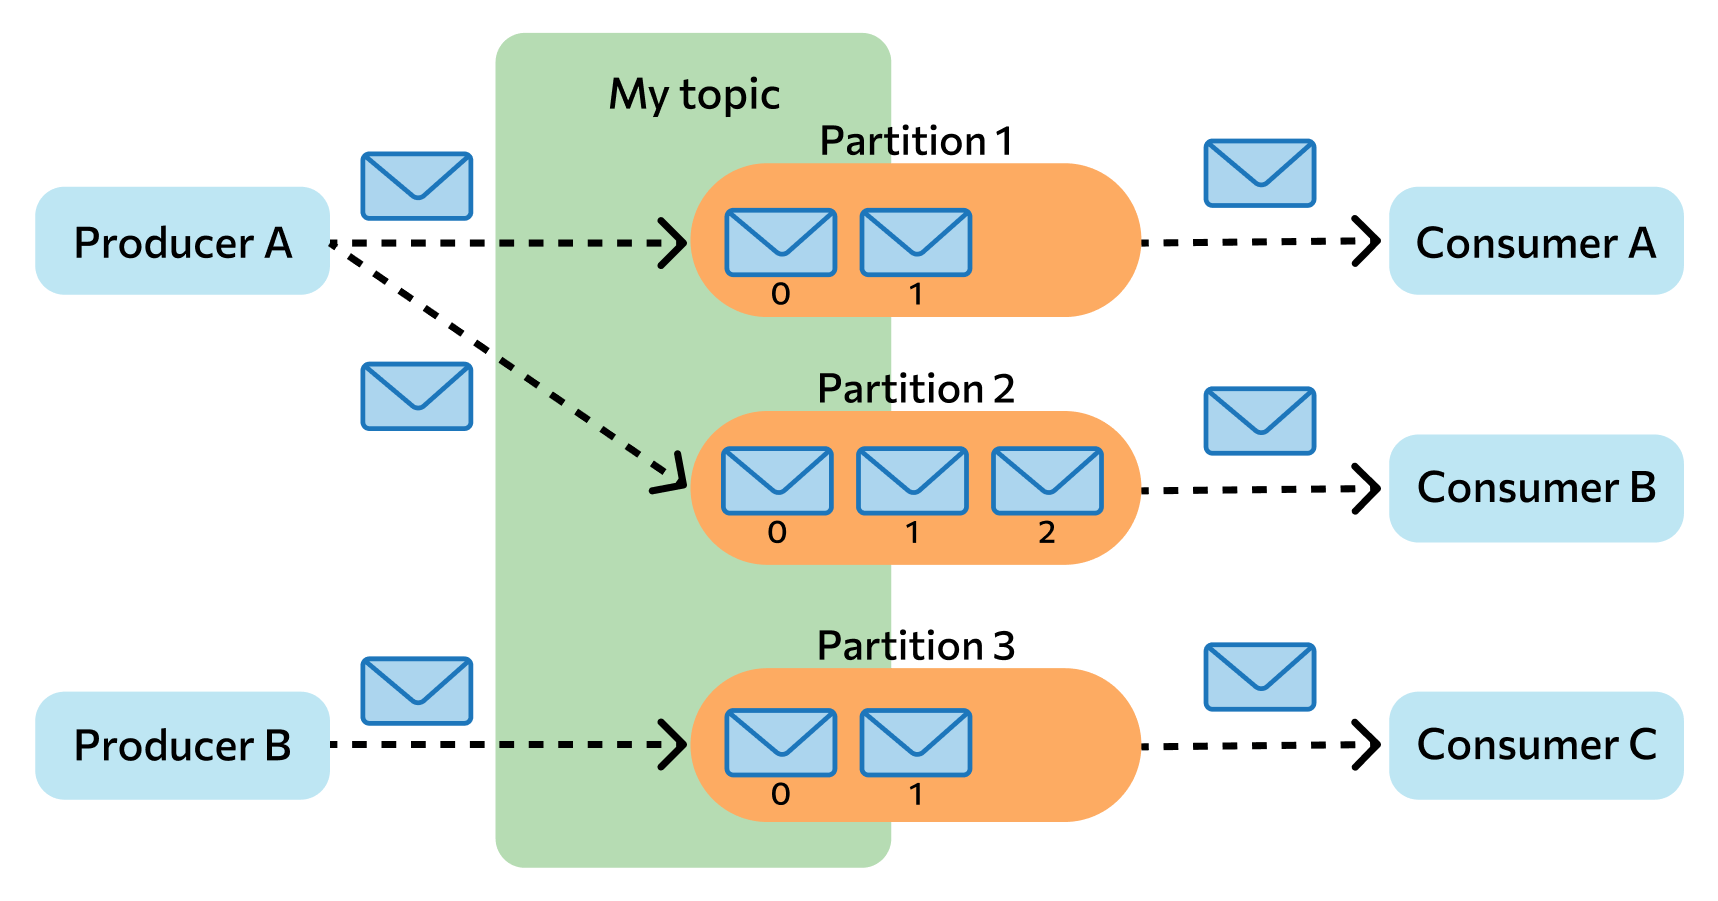
\includegraphics[width=.5\linewidth]{images/kafka_model}
    \caption{Структура Apache Kafka}
    \label{fig:domain:kafka-model}
\end{figure}

%=======================================================================================================================

\subsection{Контейнеризация}\label{subsec:domain:contenarization}
Контейнеризация -- это процесс упаковки приложения и всех его зависимостей в стандартизированный блок, называемый контейнером.
Контейнеры обеспечивают изолированную среду выполнения для приложения, что позволяет им работать независимо от среды хоста.

Контейнеризация стала популярным подходом к разработке и развертыванию приложений благодаря своей простоте, эффективности и портабельности.
Она обеспечивает множество преимуществ для разработчиков  и широко применяется в современной разработке программного обеспечения.

\subsubsection{Docker}\label{subsubsec:domain:docker}
Одной из технологий контейнеризации является Docker.
Docker представляет собой платформу для создания, управления и запуска контейнеров.

Основными сущностями в Docker являются:
\begin{itemize}
    \item Образ (Image).
    Образ можно рассматривать как набор файлов.
    В состав образа входит все необходимое для запуска и работы приложения на машине, где установлен только Docker: операционная система, среда выполнения и приложение, готовое к развертыванию.
    \item Слой (Layer).
    Образ состоит из неизменяемых слоев, каждый из которых добавляет, удаляет или изменяет файлы из предыдущего слоя.
    Неизменяемость слоев позволяет использовать их совместно в разных образах.
    \item Контейнер (Container).
    Контейнер строится на основе образа.
    Суть преобразования образа в контейнер состоит в добавлении верхнего слоя, для которого разрешена запись.
    Результаты работы приложения (файлы) пишутся именно в этом слое.
    \item Том (Volume).
    Тома обеспечивает возможность сохранения данных вне контейнера, что делает их доступными и сохраняемыми даже после остановки или удаления контейнера.
    Томы являются важной частью микросервисных архитектур, где они могут использоваться для хранения данных и других ресурсов, общих для нескольких контейнеров.
    Выделяют следующие типы томов: локальные, удаленные и именованные.
    \item Сеть (Network).
    Сеть -- это механизм, который обеспечивает коммуникацию между контейнерами и взаимодействие с внешними сетями.
    Создание собственной сети Docker позволяет контейнерам обмениваться данными, работать вместе в рамках одной сети, а также обеспечивает изоляцию и безопасность приложений.
    Docker поддерживает несколько типов сетей, включая мостовые (bridge), хостовые (host), накладные (overlay), маквланы (macvlan) и другие.
\end{itemize}

Правила создания и сборки образов описываются в специальном файле, называемом Dockerfile.
Dockerfile представляет собой набор инструкций, где каждая инструкция добавляет новый слой к образу.

\subsubsection{Docker Compose}\label{subsubsec:domain:docker-compose}
Docker Compose -- это инструмент для определения и запуска многоконтейнерных приложений.
Docker Compose позволяет определять и запускать несколько контейнеров как часть одного приложения.
Это полезно для микросервисных архитектур, где каждый сервис представлен отдельным контейнером.

Для описания конфигурации приложения используется YAML-файл с названием docker-compose.yaml.
С помощью Docker Compose можно определить:
\begin{itemize}
    \item контейнеры;
    \item тома;
    \item сети.
\end{itemize}

Docker Compose предоставляет команды для управления многоконтейнерным приложением, такие как запуск, остановка, перезапуск, масштабирование и удаление контейнеров,
что позволяет упростить процесс развертывания и управления приложением.



%\subsection{Трейдинговая платформа}

%\begin{figure}[ht]
%    \centering
%    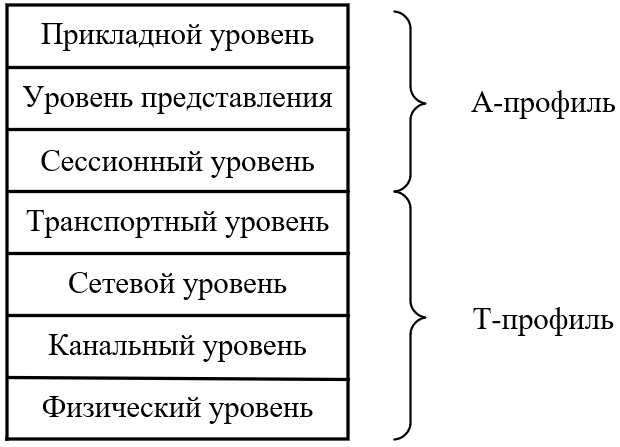
\includegraphics[width=.5\linewidth]{osiModel}
%    \caption{Эталонная модель и профили OSI}
%    \label{pic::domain::osi_model}
%\end{figure}
%как изображено на рисунке~\ref{pic::domain::osi_model}. А-профиль OSI --


% \subsection{Существующие аналоги}

% TODO: implement
